\documentclass[a4paper,11pt]{article}

\usepackage{graphicx}
\usepackage{subfig,hyperref}
\newcommand{\HRule}{\rule{\linewidth}{0.5mm}}

\begin{document}
\pagenumbering{alph}
\begin{titlepage}
\begin{center}

\textsc{\LARGE CMSC726 Machine Learning}\\[1.5cm]

\textsc{\Large Project 3}\\[0.5cm]

\HRule \\[0.5cm]

{ \huge \bfseries Unsupervised Learning}\\[0.4cm]

\HRule \\[1.5cm]

{\large Angjoo Kanazawa, Ran Liu, and Austin Myers}

\vfill

{\large December 6, 2011}

\end{center}
\end{titlepage}
\pagenumbering{arabic}

\section{PCA and Kernel PCA}
\subsection{WU1}
\textsf{Depending exactly on your random data, one or more of these lines might
not pass exactly through the data as we would like it to. Why not?}\vspace{0.1in}

\subsection{WU2}
\textsf{Plot the normalized eigenvalues (include the plot in your writeup). 
How many eigenvectors do you have to include before you've accounted 
for 90\% of the variance? 95\%? (Hint: see function cumsum.)}\vspace{0.1in}

% \begin{figure}[!ht]
%   \begin{center}
%   \caption{Plot of the normalized eigenvalues}
%   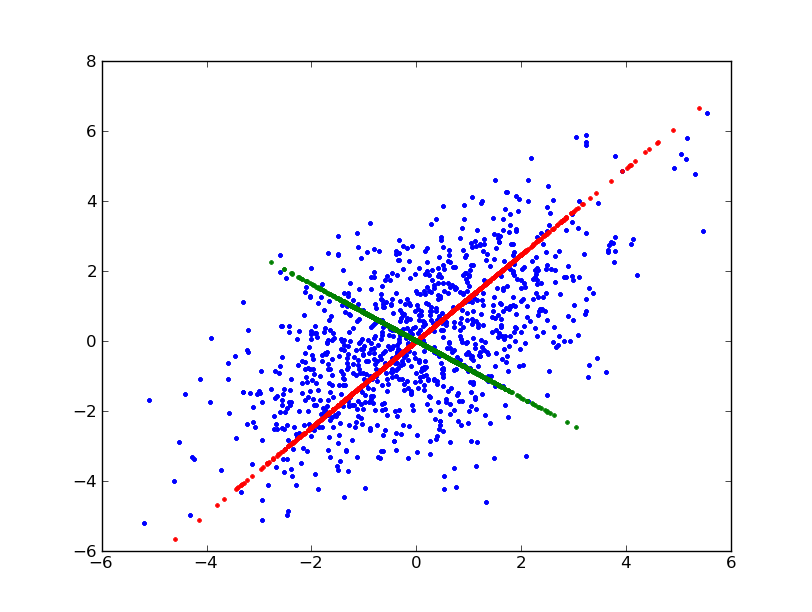
\includegraphics[width=4.5in]{pca.png}
%   \label{figures:wu61}
%   \end{center}
% \end{figure}

\subsection{WU3}
\textsf{Do these look like digits? Should they? Why or why not?
(Include the plot in your write-up.)}\vspace{0.1in}

% \begin{figure}[!ht]
%   \begin{center}
%   \caption{Plot of digits using vanilla pca}
%   \includegraphics[width=4.5in]{pca_digits.png}
%   \label{figures:wu61}
%   \end{center}
% \end{figure}

\subsection{WU4}
\textsf{Why does vanilla PCA find this data difficult? What is the
significance of the relatively large value of the eigenvalues
here?}\vspace{0.1in}
Vanilla PCA can only deal with data that is linearly separable. In this dataset, the data is not linearly separable, so vanilla PCA cannot handle it well. 
The eigenvalues are large in both directions, that is, the variance is large in both directions. Neither of the eigenvectors maximize the variance of the data. This is consistence with the data plot, where the data is in a circle. So none of the directions linear PCA gives us is significantly better than the other.  



\subsection{WU5}
\textsf{Did PCA do what we might want it to? Why or why not? Include
the plot to justify your answer.}\vspace{0.1in}

% \begin{figure}[!ht]
%   \begin{center}
%   \caption{Pca doing what we want..}
%   \includegraphics[width=4.5in]{pca2.png}
%   \label{figures:wu61}
%   \end{center}
% \end{figure}

\subsection{WU6}
\textsf{How do the eigenvalues here compare to the linear case? What
does this tell you? How does the plot look? How might this be useful
for supervised learning?}\vspace{0.1in}
The eigenvalues seperates data into two
seperate clusters better than the linear case. This is useful for
supervised learning because then since we konw the lables, we can try
different kernels, use the one that gives us the largest margin to
make the training data seperable, then train discriminative
classifiers on the data. It allows us to make linearly inseperable
data into seperable ones before we feed it to a classifier.
% \begin{figure}[!ht]
%   \begin{center}
%   \caption{Using KPCA}
%   \includegraphics[width=4.5in]{pca2.png}
%   \label{figures:wu61}
%   \end{center}
% \end{figure}

\subsection{WU7}
\textsf{Experiment with different kernels, and perhaps interpolations 
of different kernels. Try to find a kernel that gets as much of the 
variance on the first two principle components as possible. Report your 
kernel and a plot of the data projected into 2d under that kernel.}\vspace{0.1in}
$rbf0_2$ does well so far.
\pagebreak
\section{HMMs:Viterbi}
\subsection{WU8}
\textsf{Find two different observation sequences of length four that
differ only in one place, but differ in more than one place in the
guessed output.}\vspace{0.1in}

%hmm.viterbi(array([0,1,1,1]), a, b, pi) # 0 0 0 0
%hmm.viterbi(array([0,1,2,1]), a, b, pi) # 0 0 1 1

One example of this effect can be found with observation sequences
[0,1,1,1] and [0,1,2,1] which differ only in the third observed emission,
but which yield predictions of [0,0,0,0] and [0,0,1,1] respectively.
Thus, the predictions differ in two states where the observations only
differ in one.

\section{HMMs:Forward-backward}
\subsection{WU9}
\textsf{Why does EM settle in this configuration? What is it saying? 
What happens when you use three states instead of two? 
What's the resulting probability of the data? 
What about four states? What happens and why?}\vspace{0.1in}
EM settles in this configuration because it is a local minima. The
$\hat \pi = [1,0,0]$ means that we always start at state 0. We also get $P(X_t=0|X_{t-1}=0)= 0$,
i.e. when we transition we always go to a different state. All
together the results say that states alternate and that is the most
likely state sequences.

If we use three states instead of two, similar behavior happens with
$\hat \pi$. One state has a probability of 1 and the rest gets 0. But
in the transition probability, we do get a single state that
has positive probabilities for more than one states.

When we increase the states to four, the behavior is still similar in
a way that we have very high probabilities for specific transitions
and emissions, but the probability of transition is more distributed.

This is because the way we produce the intial HMM is random. When
there are only two states, the only way for the final probabilities to
be well distributed is if initial transition from state 0 to state 0
and state 0 to state 1 is close i.e. 1/2, 1/2. If anything, it's very
easy for EM to exaggerate the probability of the bigger one.

But as the number of states increases, the likelihood of uniformly
distributin the initial HMM probabilities increases. So we get more
reasonable (unskewed) results for EM.

\subsection{WU10}
\textsf{Run EM on this data using two states. 
Run it a few times until you get a final log probability at least -9250. 
(It should happen in two or three trials. This will take a few minutes to run.) 
When you do this, it will print out the resulting initial state probabilities, 
transition probabilities and emission probabilities. 
What has it learned? Include all of this output in your
write-up.}\vspace{0.1in}
The output of EM om this data is:
\begin{verbatim}
Initial state probabilities:
	state(0):	7.4252e-202
	state(1):	1

Transition probabilities:
FROM\TO
	0 	1 
0 	0.245207 	0.754793 
1 	0.720637 	0.279363 

Emission probabilities:
	State 0:
		_  0.362509
		e  0.232741
		a  0.125778
		o  0.120613
		i  0.104855
		u  0.04369
		y  0.00345083
		t  0.00258696
		k  0.0019353
		q  0.00121219
		g  0.000467752
		s  0.000115461
		c  2.34141e-05
		p  1.62641e-05
		l  3.6812e-06
		d  1.16317e-06
		b  1.69503e-07
		h  1.26829e-08
		w  8.21573e-12
		r  1.47438e-14
		f  5.26943e-15
		m  4.67596e-15
		j  2.11457e-16
		n  2.45545e-17
		x  4.24731e-29
		v  3.78819e-34
		z  3.08129e-51
	State 1:
		t  0.141537
		r  0.102944
		n  0.0971604
		s  0.0970502
		h  0.094847
		d  0.0670858
		l  0.0636134
		c  0.0479795
		m  0.0439535
		f  0.0347001
		y  0.0337207
		p  0.0329496
		w  0.0306518
		b  0.0260249
		g  0.0244221
		v  0.0202417
		k  0.0166601
		_  0.0155547
		a  0.00316851
		x  0.00173501
		j  0.00173501
		u  0.00168636
		z  0.000578336
		o  2.52571e-07
		e  6.20806e-09
		i  2.8181e-11
		q  1.18265e-17
\end{verbatim}

It has learned the probability of spaces and vowels vs the probability
of consonants! State 0 emits all spaces or vowels and state 1 emits
consonants. It also makes sense that the transition from state 0 to
state 0 is lower than that of state 1, because it's more likely that
consonants are followed by consonants than that vowels are followed by vowels.
\end{document}
